\chapter{Cascade system performance evaluation}
\section{System description}

In Section~\ref{sec:sst}, two typical cascade system topologies (see Figure~\ref{fig:CascadeSystems}) are selected for further investigation. It has to be pointed out that, in Chapter~\ref{cha:osgs}, multi-stage exergy loss reduction system (MELRS) is proposed and analyzed. It is obvious that MELRS has better energy and exergy performance than SGSS. However, the MELRS is not applied in this chapter for investigation. There are several reasons. First,
in order to clearly find out the advantages of cascade collection and cascade utilization of the cascade systems, it is not applied in the cascade system in this chapter. Second, compared with traditional SGSS, MELRS only changes the solar field, which has no influence on the cascade utilization of the cascade system. It can be easily applied in the cascade system analyzed in this chapter in the future without influence of existing calculations. Third, the MELRS proposed in Chapter~\ref{cha:osgs} needs further research in the future. Different types of solar collector technologies can be applied in different solar fields. For example, linear Fresnel reflectors or flat collectors can be applied for the preheating solar field to reduce costs; molten salt can be used as heat transfer fluid in the superheating solar field to increase the main steam temperature of the Rankine cycle.

Two typical cascade system topologies are selected in Chapter~\ref{cha:SystemTopology}. 
Both systems take advantage of the different types of heat collectors and different thermal cycles to achieve cascade collection of energy and cascade utilization.
However, this chapter focuses on the first model because it is more widely used and more suitable for large-scale applications. 
Figure~\ref{fig:System-1} shows the scheme sketch of the cascade system.
In this system, dish collectors are used to provide heat for Stirling engines and air-to-water heat exchanger. Trough collectors are used to provide heat for steam generating processes (preheating, evaporating and superheating) in the Rankine cycle. Hot air is produced by the dish collectors. High temperature (1073\,K) air is used to provide heat to Stirling cycle to get higher conversion efficiency, then the air is used to provide heat for air-to-water heat exchanger to use the lower temperature energy in Rankine cycle effectively. Besides, feed water of Rankine cycle is used to cool the Stirling engines to recycle the heat wasted conventionally. The Stirling engines are connected in series for better performance.
%Water is used as the working fluid of Rankine cycle, which is heated in the cold chamber of Stirling engines, preheater, evaporator, superheater, and air-to-water heat exchanger successively, and then expand in turbine, condense in condenser. Pumps are used to change the pressure of fluids. Stirling engines are used for power generation and cooled by feed water of the Rankine cycle. 

\noindent \begin{figure}[htbp]
\begin{center}
	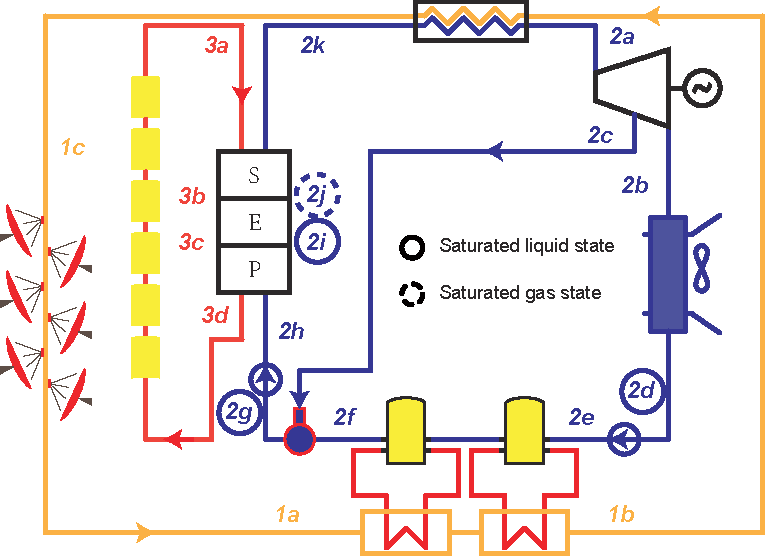
\includegraphics[width = 0.8\columnwidth]{fig/cascadeSystem}
	\caption{Sketch of the cascade system}
	\label{fig:System-1}
\end{center}
\end{figure}

Figure~\ref{fig:T-s_Water2} shows the $T$-$s$ diagram of the water circuit in the cascade system. In this Rankine cycle, the heat provided in process $2e$-$2f$ comes from the Stirling engines, which increases the power of Rankine cycle. Figure~\ref{fig:HeatTransfer_Water-SEs} shows the heat transfer diagram of this process.

\noindent \begin{figure}[htbp]
\centering
	\begin{subfigure}[b]{0.45\columnwidth}
	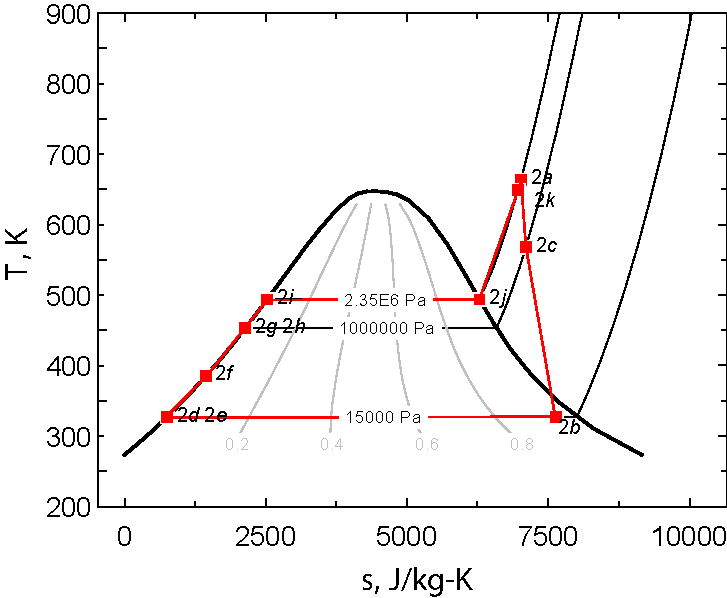
\includegraphics[width = \columnwidth]{fig/T-s_Water2}
	\caption{$T$-$s$ diagram of the water circuit}\label{fig:T-s_Water2}
	\end{subfigure}
	~
\begin{subfigure}[b]{0.45\columnwidth}
	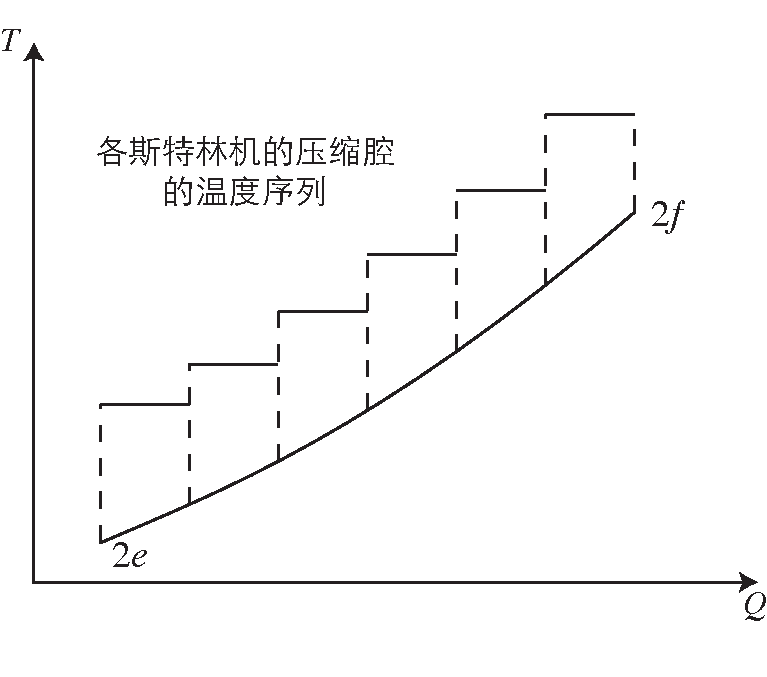
\includegraphics[width = \columnwidth]{fig/HeatTransfer_Water-SEs}
	\caption{Diagram of process $2e$-$2f$}\label{fig:HeatTransfer_Water-SEs}
	\end{subfigure}
	
	\caption{Diagrams of water circuit and $2e$-$2f$ process}\label{fig:Diagrams$2e$-$2f$}
\end{figure}


%\noindent \begin{figure}[htbp]
%\begin{center}
%	\subfigure[$T$-$s$ diagram of the water circuit]{
%	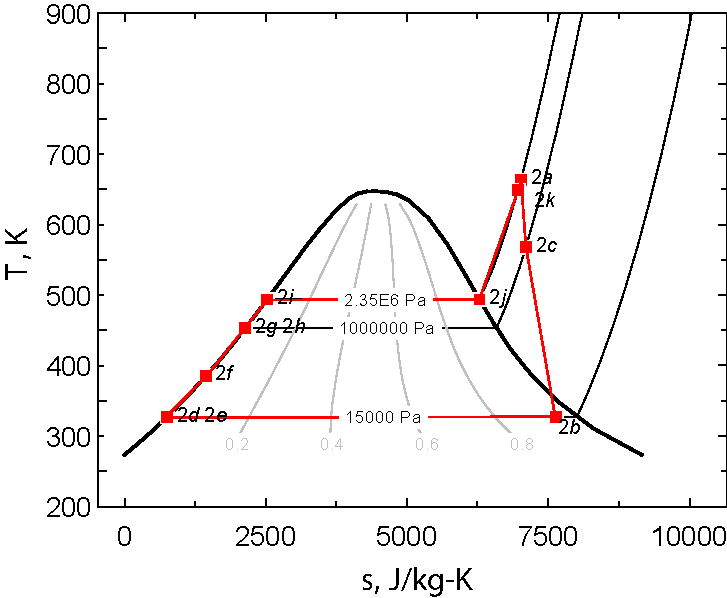
\includegraphics[width = 0.4\columnwidth]{fig/T-s_Water}
%	\caption{$T-s$ diagram of the water circuit}
%	\label{fig:T-s_Water}}
%	~\subfigure[Heat transfer diagram of process $2e$-$2f$]{
%	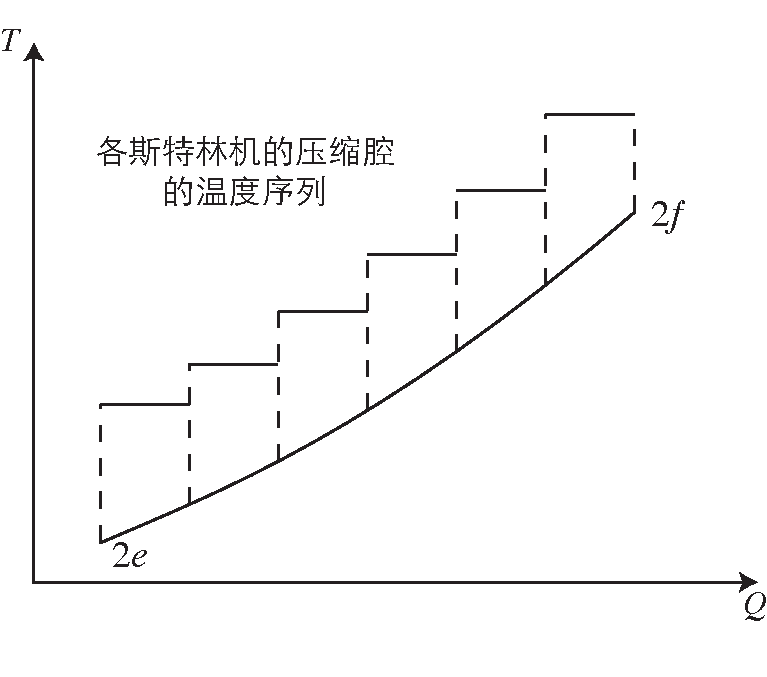
\includegraphics[width = 0.4\columnwidth]{fig/HeatTransfer_Water-SEs}
%	\caption{Heat transfer diagram of process $2e$-$2f$}
%	\label{fig:HeatTransfer_Water-SEs}}
%	\caption{Diagrams of water circuit and $2e$-$2f$ process}
%\end{center}
%\end{figure}

%\noindent \begin{figure}[htbp]
%\begin{center}
%	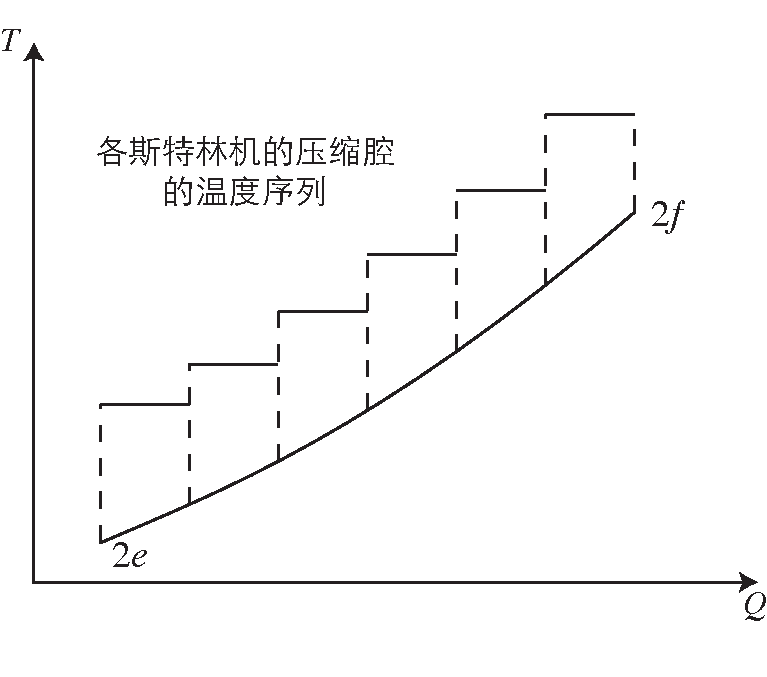
\includegraphics[width = 0.7\columnwidth]{fig/HeatTransfer_Water-SEs}
%	\caption{Heat transfer diagram of process $2e$-$2f$}
%	\label{fig:HeatTransfer_Water-SEs}
%\end{center}
%\end{figure}

To build the cascade system model, several simplifying assumptions are made:

\begin{itemize}
	\item Steady state at nominal load of the system is analysed.
	\item Pressure drop due to flow is negligible.
	\item The leak of working fluid in the pipes is neglected.
	\item Same isentropic efficiency of steam turbine with different loads and in different stages.
	\item Heat loss that occurs from the tube to the atmosphere is not considered.
	\item There is no heat loss to the environment for Stirling engines.
	\item Simple models are used of some processes and equipment.
	\item A symmetrical regenerator behavior is assumed so that a single effectiveness can be defined as $e = (T_R - T_L) /(T_H - T_L)$.~\cite{Formosa2010, Juhasz2010}
	\item A linear temperature profile across the regenerator exists, the mean effective temperature $T_{R} = (T_H-T_L) / \ln(T_H/T_L)$.~\cite{Der2007, Cavazzuti2012}
\end{itemize}

\section{System parameters}

In order to study the efficiency of the system and its influencing factors, a model of the cascade system is required. Chapter~\ref{cha:Modeling} introduces the system modeling process in detail. After the system modeling process, another important task is to determine the system parameters.

The system mainly consists of the following components:

\subsection{Environment}

Typical environmental parameter values of Wuhan are used for the cascade system design.

$I_r = 700\,\mathrm{W/m^2}$, $T_{amb} = 293\,\mathrm{K}$, $p_{amb} = 1\times10^5\,\mathrm{Pa}$, $v_{amb} = 1\,\mathrm{m/s}$.

\subsection{Steam Turbine} 
	
A steam turbine product, N-6 2.35, of Qingdao Jieneng Power Station Engineering Co., Ltd is used for calculation. Its nominal parameters are: $P = 6\,\mathrm{MW}$, 	$p_s = 2.35\,\mathrm{MPa}$, $T_s = 390\mathrm{^\circ C}$, $\dot{m} = 32.09\,\mathrm{t/h}$, $p_c = 0.015\,\mathrm{MPa}$, $s_{tb} = 3000\,\mathrm{rpm}$.
	
	Known the main steam parameters, its enthalpy and entropy can be obtained by using CoolProp, $h_s = 3.2203\times10^6\,\mathrm{J/kg}$, $s_s = 7.0149\times10^3\,\mathrm{J/(kg\cdot K)}$.
	
	Exhaust enthalpy of the turbine $h_{c} = h_{s} - \dfrac{P}{\dot{m}} = 2.5472\times10^6\,\mathrm{J/kg}$.
	
	Known exhaust pressure and $s_{i,c} = s_s$, isentropic exhaust enthalpy of the turbine can be obtained by using CoolProp, $h_{i,c} = 2.2737\times10^6\mathrm{J/kg}$.	
	
	So the isentropic efficiency of the turbine can be obtained from
	$\eta_{i,tb} = \dfrac{h_s - h_c}{h_{s} - h_{i,c}} = 0.71$.
	
	Taking into account of the application in solar trough system, the designed parameters of the steam turbine are shown in Table~\ref{tab:CascadeSystemParameters}.
		 
\subsection{Trough collector}
LUZ solar collector LS-3 is used as the trough collector for its known test data. Its main characters are listed in Table~\ref{tab:TroughParameters}~\cite{Fernandez2010}.

\begin{table}[htbp]
	\caption{Main parameters of LS-3}
	\begin{center}
	\begin{tabular}{cccccc}
		\toprule
		Parameter		&	Value	&	Parameter		&	Value	&	Parameter		&	Value\\
		\midrule
		$A_{pc}$		&	$570.2\,\mathrm{m^2}$	&	$w_{dc}$	&	$5.76\,\mathrm{m}$	&	$L_{dc}$	&	$99\,\mathrm{m}$\\
		$f$	&	$1.71\,\mathrm{m}$	&	$d_i$		&	$0.066\,\mathrm{m}$	&	$d_o$	&	$0.07\,\mathrm{m}$\\
		$d_{abs,i}$	&	$0.113\,\mathrm{m}$	&	$d_{abs,o}$	&	$0.115\,\mathrm{m}$	&	Rim angle	&	$80^\circ$\\
		$\epsilon$		&	$0.15$	&	$\eta_{peak}$	&	$0.77$	&	$\rho$	&	$0.94$\\
		$\tau$	&	$0.95$	&	
$\alpha$	&	$0.96$	&	$Fe$	&	$0.97$\\
		\bottomrule
	\end{tabular}
	\end{center}
	\label{tab:TroughParameters}
\end{table}
\nomenclature{$f$}{Focal length, m}

\subsection{Dish collector}
A dish reflector product of SES (Stirling Energy System) is used as the reflector, the receiver is self-designed. The key parameters of the dish collector are listed in Table~\ref{tab:dc}. 

\subsection{Stirling engines}
The Stirling engines used in the cascade system are the same with the one analyzed in Section~\ref{sec:StirlingEngineModel}. It is a GPU-3 type Stirling engine, Table~\ref{tab:GPU3parameters} shows its parameters.

\subsection{Preheater}
Water is heated to saturated water in the preheater by the oil. For outlet stream of water, $x = 0$.
Besides, considering the minimum temperature difference required between oil and water, $T_{3c} - T_{2i} = \Delta T_{3,2,min}$. $\Delta T_{3,2,min}$ is set to be $15\,\mathrm{K}$.

\subsection{Evaporator}
Water is heated from saturated liquid water to saturated steam in the evaporator. For outlet stream of water, $x = 1$.

\subsection{Superheater}
The inlet temperature of oil is limited by the oil properties. In the cascade system, Therminol VP-1 Synthetic oil is used as the heat transfer fluid. Its properties can be obtained from both EES and CoolProp. The inlet temperature of the oil of superheater is set as $T_{3a} = 623\,\mathrm{K}$.

\subsection{Deaerator}
The deaerator has two inlet streams and one outlet stream. They have the same pressure, $p_{se} = 1\times10^6\,\mathrm{Pa}$. The outlet stream of the deaerator is saturated water.

\subsection{Air-water heat exchanger}
The inlet temperature is set as $T_{1b} = 673\,\mathrm{K}$.

\subsection{Main design parameters summary}
The main design parameters of the cascade system can be concluded in Table~\ref{tab:CascadeSystemParameters}.

\begin{table}[htbp]
	\caption{Basic design parameters of the cascade system}
	\begin{center}
	\begin{tabular}{cccccc}
		\toprule
		Parameter		&	Value	&	Parameter		&	Value	&	Parameter		&	Value\\
		\midrule
		$I_r$		&	$700\,\mathrm{W/m^2}$	&	$T_{dc,o}$	&	$1073\,\mathrm{K}$	&	$n_{se}$	&	100\\
		$T_{amb}$	&	$293\,\mathrm{K}$	&	$p_{dc}$		&	$5\times10^5\,\mathrm{Pa}$	&	$T_s$	&	$613\,\mathrm{K}$\\
		$p_{amb}$	&	$1\times10^5\,\mathrm{Pa}$	&	$\Delta{}T_{3,2,min}$	&	$15\,\mathrm{K}$	&	$p_s$	&	$2.35\times10^6\,\mathrm{Pa}$\\
		$v_{amb}$	&	$1\,\mathrm{m/s}$	&	$T_{tc,o}$	&	$623\,\mathrm{K}$	&	$p_c$	&	$1.5\times10^4\,\mathrm{Pa}$\\
		$P_{ge}$	&	$6\times10^6\,\mathrm{W}$	&	
$p_{tc}$	&	$2\times10^6\,\mathrm{Pa}$	&	$T_{s,d}$	&	$663\,\mathrm{K}$\\
		$T_{dc,i}$		&	$623\,\mathrm{K}$	&	$T_{1b}$	&	$673\,\mathrm{K}$	&	$p_{de}$ 	& 	$1\times10^6\,\mathrm{Pa}$\\			
		\bottomrule
	\end{tabular}
	\end{center}
	\label{tab:CascadeSystemParameters}
\end{table}

\section{System evaluation method}

There are two aspects to be evaluated for the cascade system. The first one is the performance. The cascade system uses different types of collectors and different thermodynamic cycles. They are closely linked together. It is unable to define part of the system's efficiency or to indicate the output power of one specific kinds of collector. A common approach is to define the overall efficiency of the system. The overall solar-to-electric efficiency equals to the total output power divided by the total input solar energy. 

The other one is to compare with existing solar thermal power technologies. This requires more consideration. 

\begin{enumerate}[label=(\arabic*)]
	\item Compare with parabolic trough. 

	When compared with parabolic trough system, a higher efficiency of the cascade system may be explained as the usage of solar dish collector. It is difficult to tell if the higher efficiency is due to the usage of cascade system or	the usage of dish collector.
	\item Compare with parabolic dish.
	
	When compared with parabolic dish system, a lower cost of the cascade system may be explained as the usage of solar trough collector. It is difficult to tell if the lower cost is due to the usage of cascade system or the usage of trough collector.
	\item Compare with stand-alone systems.
	
	It is important to choose good stand-alone systems. An intuitive idea is to use both parabolic trough and parabolic dish for comparison. To compare two systems, contrast conditions needs to be set. 
	
	If the same output power was selected as the contrast condition, different amount of trough collectors and dish collectors will be used in the cascade system and stand-alone systems.
	It is complicated for cost comparison due to different prices of trough collectors and dish collectors.
	
	A better way is to select the same collectors as the contrast condition. Since the output is electricity, it is much more convenient for both efficiency comparison and cost comparison.
	
\end{enumerate}


\section{Stand-alone system selection}

\noindent \begin{figure}[htbp]
\centering
	\begin{subfigure}[b]{0.64\columnwidth}
	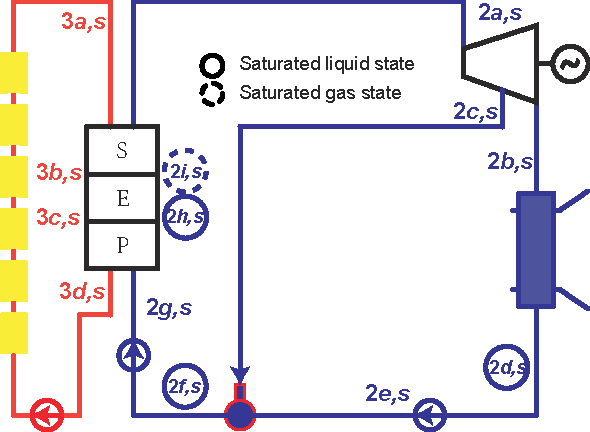
\includegraphics[width = \columnwidth]{fig/Trough-s}
	\caption{Trough-Rankine system}\label{fig:TroughRankine}
	\end{subfigure}
	~
\begin{subfigure}[b]{0.26\columnwidth}
	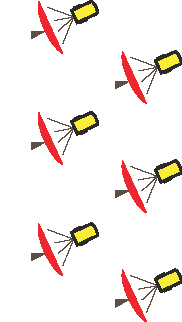
\includegraphics[width = \columnwidth]{fig/Dish-s}
	\caption{Dish-Stirling system}\label{fig:DishStirling}
	\end{subfigure}
	
	\caption{Sketch of the stand-alone systems}\label{fig:Stand-alone-systems}
\end{figure}

%\noindent \begin{figure}[htbp]
%\begin{center}
%	\subfigure[Trough-Rankine system]{
%	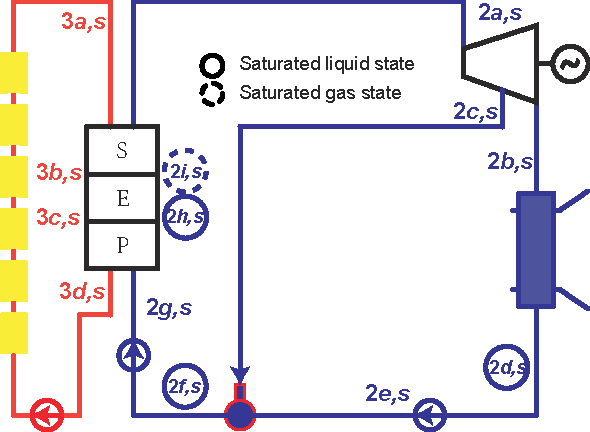
\includegraphics[width = 0.45\columnwidth, angle = 0]{fig/Trough-s}}
%	\subfigure[Dish-Stirling system]{
%	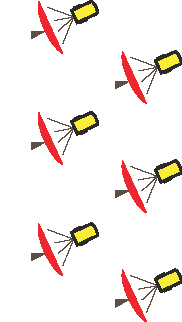
\includegraphics[width = 0.19\columnwidth, angle = 0]{fig/Dish-s}}
%	\caption{Sketch of the stand-alone systems}
%	\label{fig:Stand-alone-systems}
%\end{center}
%\end{figure}

Figure~\ref{fig:Stand-alone-systems} shows the sketch of the stand-alone systems. These two stand-alone systems were developed for comparison. They use the same dish collectors and trough collectors with the same thermal efficiencies of the cascade system.

\subsection{Stand-alone trough-Rankine system}

Steam turbine has the same main parameters and isentropic efficiency with that of the cascade system. Working pressure of deaerator is the same of the cascade system. So parameters of state $2b,s$ and $2c,s$ in Figure~\ref{fig:Stand-alone-systems} of the steam turbine can be obtained by
\nomenclature[S]{$s$}{Stand-alone systems}

\begin{equation}
	\eta_{i,tb}= (h_{2a,s}-h_{2b,s})/(h_{2a,s}-h_{i,2b,s}) = (h_{2a,s}-h_{2c,s})/(h_{2a,s}-h_{i,2c,s})
\end{equation}

The output power of steam turbine

\begin{equation}
	P_{tb,s}=\left(1-y_{s}\right)\dot{m}_{2,s}\left(h_{2a,s}-h_{2b,s}\right)+y_{s}\dot{m}_{2,s}\left(h_{2a,s}-h_{2c,s}\right)
\end{equation}

The output power of generator

\begin{equation}
	P_{ge,s}=P_{tb,s}\eta_{ge}
\end{equation}

The total power of pumps
\begin{equation}
	P_{pu,s}=\left(1-y_{s}\right)\dot{m}_{2,s}\left(h_{2e,s}-h_{2d,s}\right)+\dot{m}_{2,s}\left(h_{2g,s}-h_{2f,s}\right)
\end{equation}

Heat injected in the water circuit

\begin{equation}
	Q_{2,s}=\dot{m}_{2,s}\left(h_{2a,s}-h_{2g,s}\right)
\end{equation}

The generator efficiency is the same of that in the cascade system, and the efficiency of Rankine cycle can be expressed as

\begin{equation}
	\eta_{rk,s}=(P_{tb,s}-P_{pu,s}/\eta_{ge})/Q_{2,s}
\end{equation}

\subsection{Stand-alone dish-Stirling system}

In the stand-alone dish-Stirling system, Stirling engines with the same number of dish collectors are directly put on the focuses of the dish collectors. Water is used for cooling the Stirling engines. $T_{H,s}$ is chosen to be equal to outlet temperature of air in dish receiver. $T_{L,s}$ is chosen to be 310 K, the default expansion temperature in Fraser's dissertation~\cite{Fraser2008} for the calculation of 4-95 NK\uppercase\expandafter{\romannumeral2} engine. $k$ and $\gamma$ are chosen the same value as that of the Stirling engines in the cascade system.

\begin{equation}
	\eta_{sea,s}=\dfrac{T_{H,s}-T_{L,s}}{T_{H,s}+\dfrac{1-e_{s}}{k-1}\cdot\dfrac{T_{H,s}-T_{L,s}}{\ln\gamma}}
\end{equation}

where, $T_{R,s}=\dfrac{T_{H,s}-T_{L,s}}{\ln(T_{H,s}/T_{L,s})}$ and $e_{s}=\dfrac{T_{R,s}-T_{L,s}}{T_{H,s}-T_{L,s}}$.

The power of Stirling engines

\begin{equation}
	P_{sea,s}=n_{dc}A_{dc}I_r\eta_{dc}\eta_{sea,s}
\end{equation}
\nomenclature{$n$}{Number of collectors}

\section{Comparison with stand-alone system}
The results presented in Table~\ref{tab:importantResults} are issued using design parameters with counterflow of two fluids in Stirling engine array as the default flow type. It is shown that the cascade system with design parameters can achieve higher efficiency compared to corresponding stand-alone systems. Although the efficiency of the Stirling engine array is lower, the efficiency of the Rankine cycle is higher. The overall output power of the cascade system is $3.83\times10^4\,\mathrm{W}$ higher.
%Different results between two flow types of Stirling engine array are listed in Table~\ref{tab:SEAresults}.

\begin{table}[htbp]
	\caption{Some important results using design parameters}
	\begin{center}
	\begin{tabular}{cccccc}
		\toprule
		Parameter		&	Value	&	Parameter		&	Value	&	Parameter		&	Value\\
		\midrule
		$\eta_{cs}$		&	0.1974	&	$\eta_{sea,s}$	&	0.3786	&	$P_{ge,s}$	&	$5.826\times10^6\,\mathrm{W}$\\
		$\eta_{s}$	&	0.1962	&	$\eta_{rk}$	&	0.2660	&	$P_{sea}$		&	$3.552\times10^5\,\mathrm{W}$\\
		$\eta_{diff}$		&	0.0062	&	$\eta_{rk,s}$	&	0.2678	&	$P_{sea,s}$	&	$4.909\times10^5\,\mathrm{W}$\\
		$\eta_{sea}$	&	0.3407	&	$P_{ge}$		&	$6\times10^6\,\mathrm{W}$	&	$P_{diff}$		&	$3.830\times10^4\,\mathrm{W}$\\
		\bottomrule
	\end{tabular}
	\end{center}
	\label{tab:importantResults}
\end{table}
\nomenclature[S]{$cs$}{Cascade system}
\nomenclature[S]{$se$}{Stirling engine}
\nomenclature[G]{$\eta_{diff}$}{Efficiency difference of cascade system and stand-alone systems, $\eta_{cs}-\eta_{s}$}
\nomenclature[S]{$sea$}{Stirling engine array}
%\nomenclature{$P_{sea,s}$}{Total power of Stirling engines in stand-alone dish system, W}

\subsection{Effects of $I_{r}$}
\label{sec:I_r}

It is found that $I_r$ can affect the efficiency difference of cascade system and stand-alone systems $\eta_{diff}$. Figure~\ref{fig:I_r-eta_diff} shows curve fits of efficiency differences $\eta_{diff}$ versus $I_r$ with a series of different Stirling engine array power ratios. As it can be seen, for a high $I_r$ ($I_r > 550\,\mathrm{W/m^2}$), $\eta_{diff}>0$, the cascade system can achieve a higher efficiency than corresponding stand-alone systems. For a low $I_r$ ($I_r < 550\,$W/m$^2$), $\eta_{diff}$ may be negative. At this situation, the cascade system achieves a lower efficiency than corresponding stand-alone systems. This may be explained that instead of cooling water in the stand-alone dish-Stirling system, condensed water of Rankine cycle is used to cool the Stirling engines, which jeopardizes the heat dissipation and leads to a lower power of the Stirling engines. For a low $I_r$, the increased power of steam turbine due to absorbed heat by the condensed water is lower than the power loss of the Stirling engines. It can also be found that higher $I_r$ can achieve higher $\eta_{diff}$, which can be interpreted as the heat absorbed by the condensed water increases with $I_r$. So a higher $I_r$ location is always more suitable for cascade system. This means $I_r$ is a key factor to determine whether cascade system should be applied in a certain location.
\nomenclature[G]{$\beta$}{Ratio of power of Stirling engines to the total output power of cascade system}

\noindent \begin{figure}[htbp]
\begin{center}
	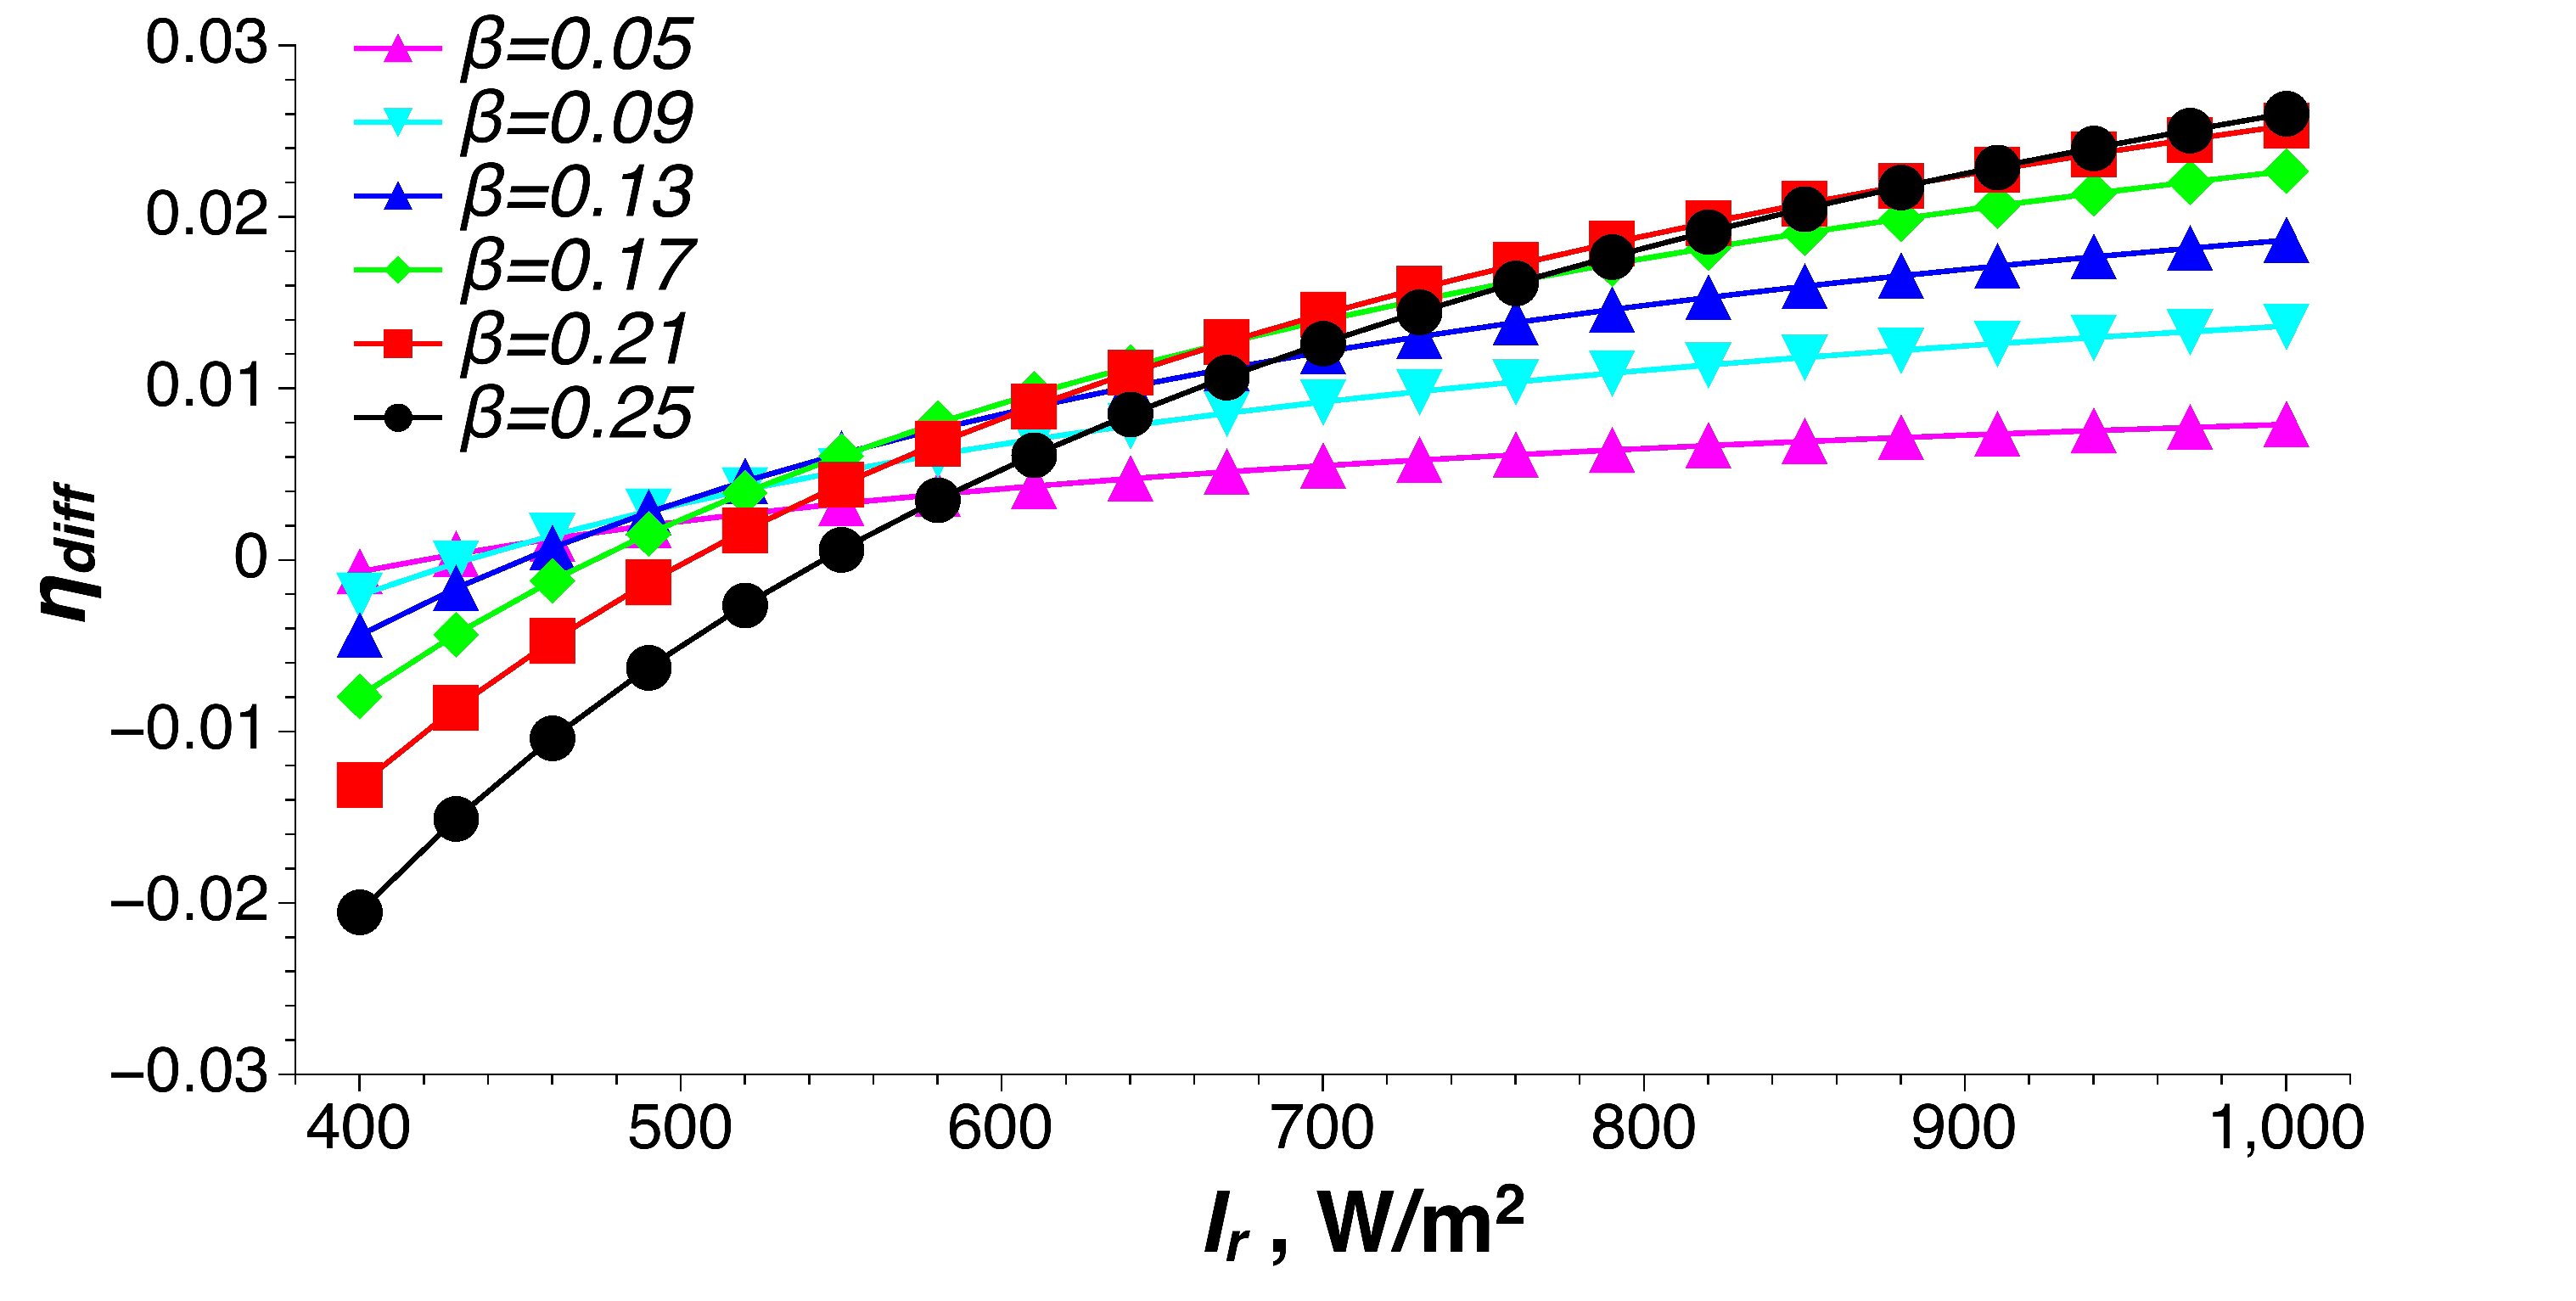
\includegraphics[width = 0.8\columnwidth, angle = 0]{fig/I_r-eta_diff}
	\caption{Curve fits of efficiency difference $\eta_{diff}$ versus $I_r$}
	\label{fig:I_r-eta_diff}
\end{center}
\end{figure}

\subsection{Effects of $\beta$}

As it can be seen in Table~\ref{tab:importantResults}, the $\eta_{diff}$ is very small with the design parameters given above. A reason $\eta_{diff}$ to be so small is that $\beta$, the ratio of power of Stirling engines to the total power, is very small, the heat released by the Stirling engine array is a small portion of the heat absorbed in the Rankine cycle. So increase $\beta$ may achieve higher $\eta_{diff}$. The relationship between $\eta_{diff}$ and $\beta$ under a series of $I_r$ is shown in Figure~\ref{fig:beta-eta_diff}. It can be found that, for a high $I_r$, increase $\beta$ may achieve a higher $\eta_{diff}$, but there is a limit. For $I_r=900$W/m$^2$, the maximum $\eta_{diff}=0.0228$ appears at $\beta=0.23$. For a low $I_r$, $\eta_{diff}$ is negative, increase $\beta$ will reduce $\eta_{diff}$. This can be explained as the same reason in Section~\ref{sec:I_r}.

\noindent \begin{figure}[H]
\begin{center}
	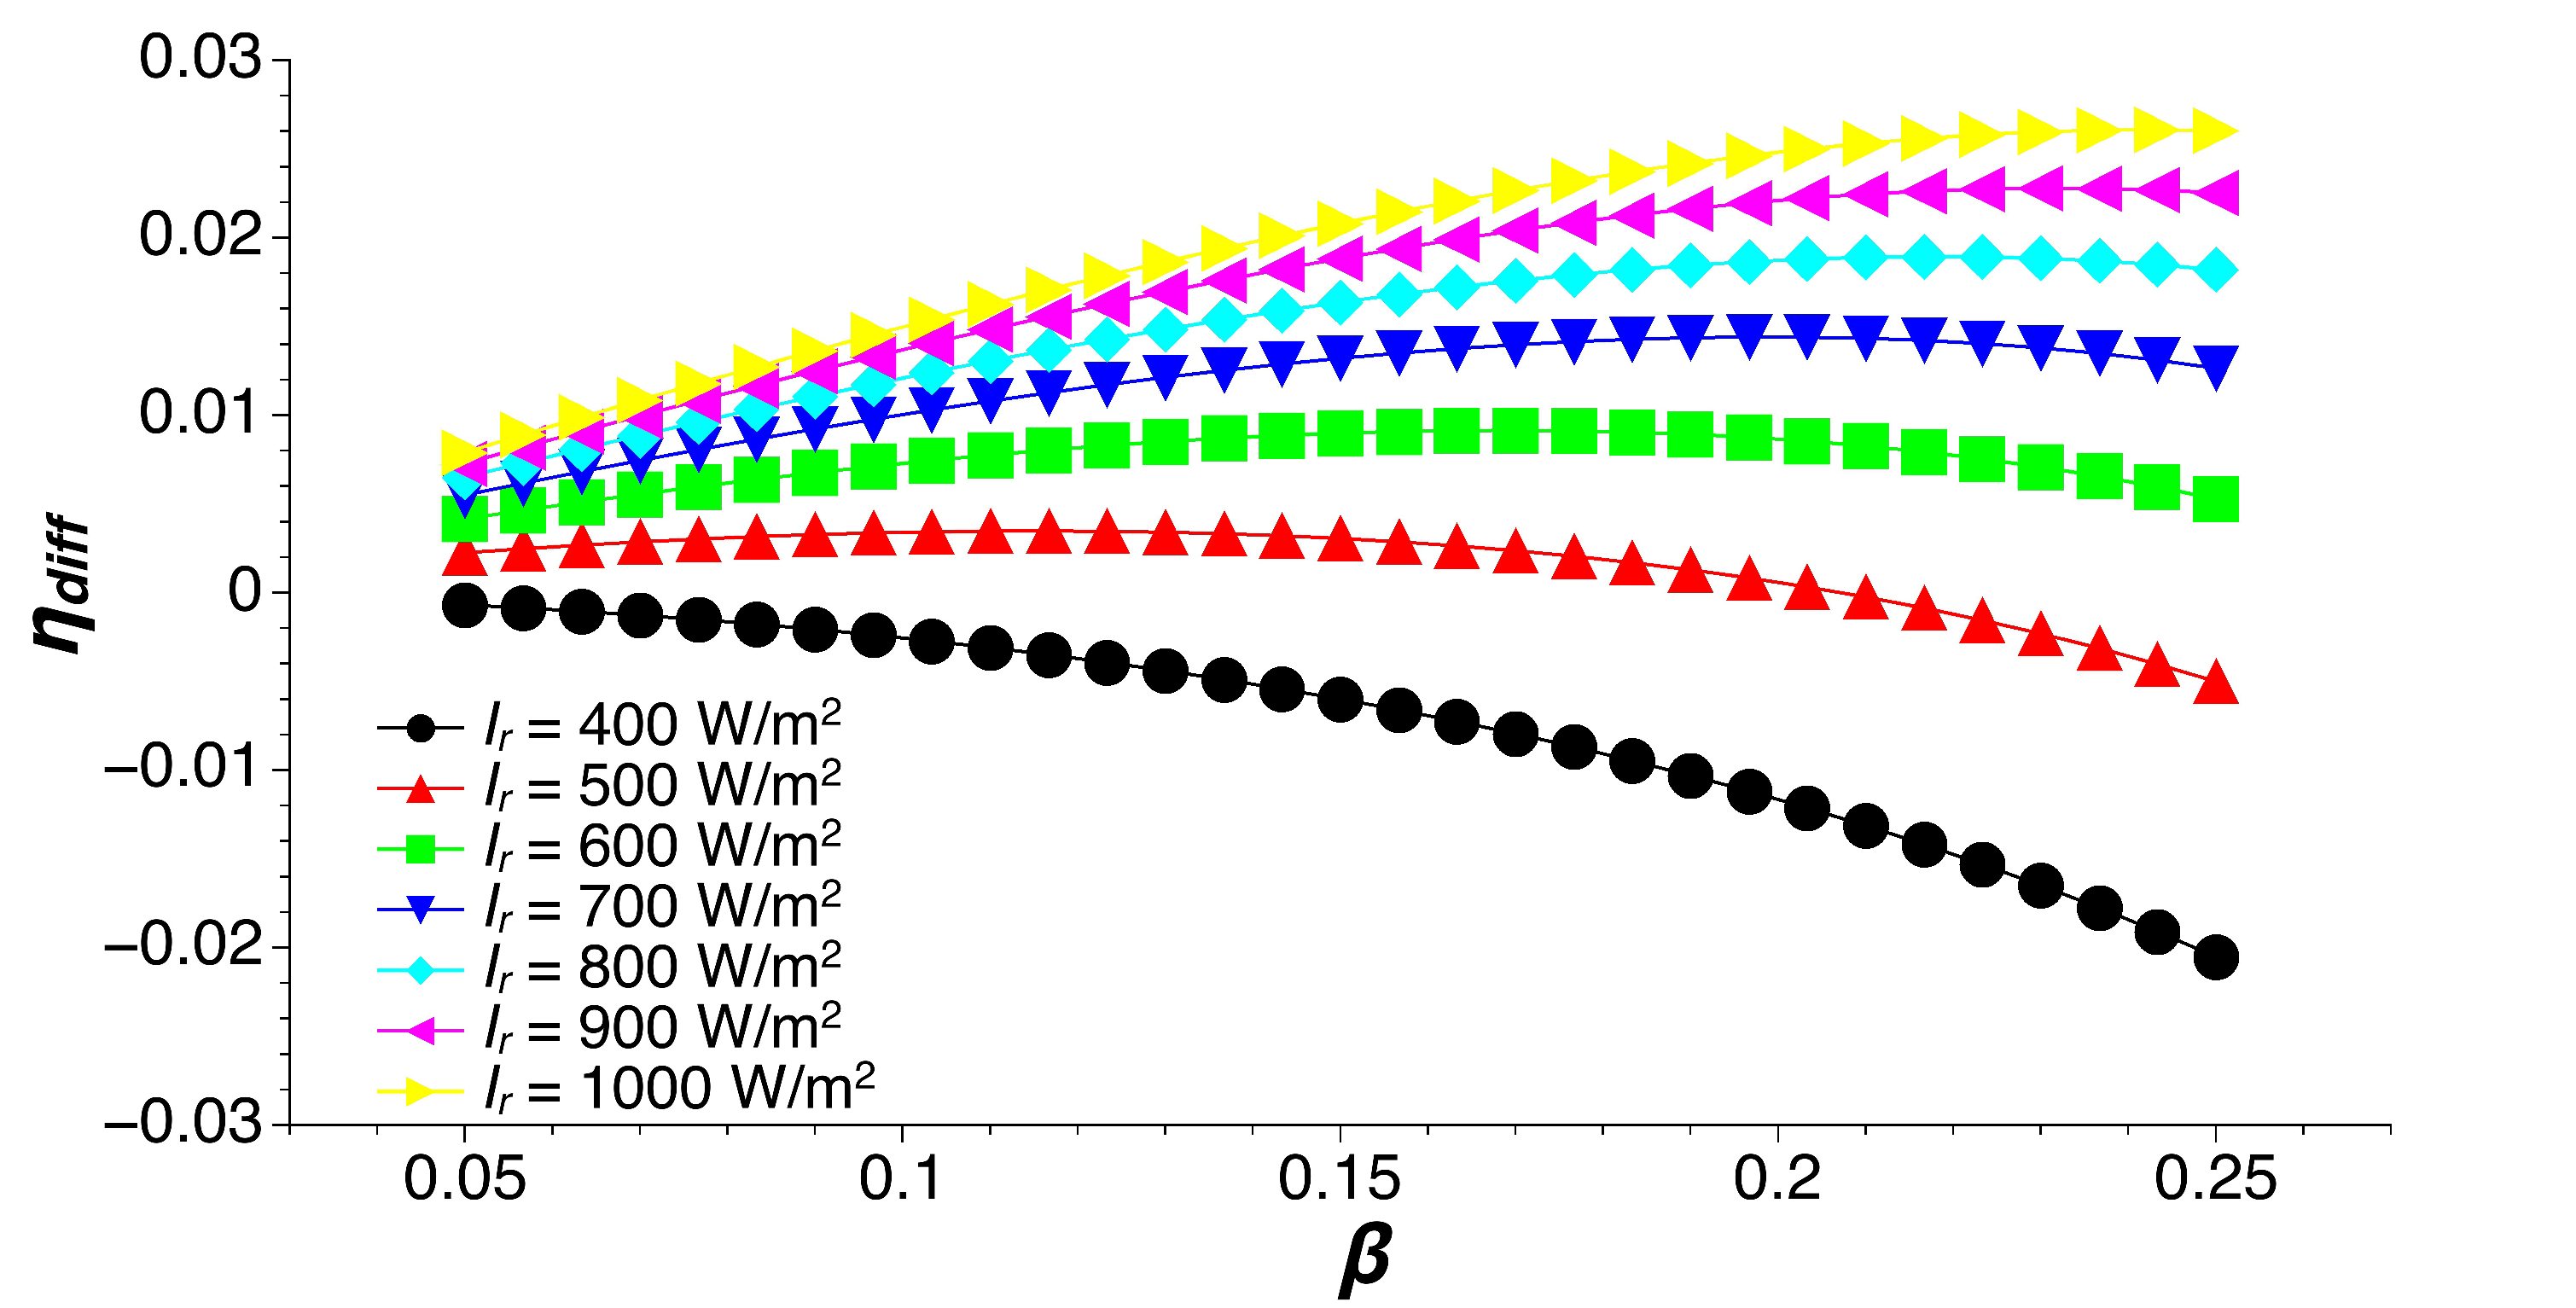
\includegraphics[width = 0.8\columnwidth, angle = 0]{fig/beta-eta_diff}
	\caption{Curve fits of efficiency difference $\eta_{diff}$ versus $\beta$}
	\label{fig:beta-eta_diff}
\end{center}
\end{figure}

\subsection{Effects of flow type}

Flow type between heating and cooling streams can affect the efficiency of Stirling engine array. Parallel flow, compared to counterflow, leads to higher Stirling engine efficiency in the first columns of the array for lower cooling temperature, while lower Stirling engine efficiency in the last columns for higher cooling temperature. 

\begin{table}[htbp]
	\caption{Results of Stirling engine array with two different flow types}
	\begin{center}
	\begin{tabular}{ccccccccc}
		\toprule
		\multirow{3}{*}{$x$}	&	\multicolumn{4}{c}{Parallel flow}	&\multicolumn{4}{c}{Counterflow}\tabularnewline
		\cline{2-5}	\cline{6-9}
		&$T_{1,i}$&$T_{2,i}$&$P_{sea}$&$\eta_{sea}$&$T_{1,i}$&$T_{2,i}$&$P_{sea}$&$\eta_{sea}$\tabularnewline
		&K&K&W&-&K&K&W&-\tabularnewline
		\midrule
		1	&	1073.15	&	327.17	&	5000	&	0.3648	&	1073.15	&	348.09	&	4867	&	0.3601\\
		2	&	1022.38	&	329.80	&	4630	&	0.3599	&	1023.25	&	345.48	&	4541	&	0.3562\\
		3	&	974.35	&	332.29	&	4280	&	0.3544	&	975.82	&	343.00	&	4230	&	0.3520\\
		4	&	928.90	&	334.65	&	3949	&	0.3485	&	930.75	&	340.65	&	3934	&	0.3474\\
		5	&	885.91	&	336.88	&	3635	&	0.3419	&	887.94	&	338.42	&	3654	&	0.3424\\
		6	&	845.26	&	339.00	&	3338	&	0.3347	&	847.28	&	336.29	&	3387	&	0.3370\\
		7	&	806.82	&	341.00	&	3057	&	0.3269	&	808.69	&	334.28	&	3134	&	0.3312\\
		8	&	770.49	&	342.91	&	2792	&	0.3184	&	772.06	&	332.37	&	2894	&	0.3248\\
		9	&	736.16	&	344.71	&	2541	&	0.3090	&	737.31	&	330.55	&	2666	&	0.3180\\
		10	&	703.75	&	346.43	&	2304	&	0.2989	&	704.37	&	328.82	&	2450	&	0.3106\\
		\bottomrule
	\end{tabular}
	\end{center}
	\label{tab:SEAresults}
\end{table}

Table~\ref{tab:SEAresults} shows the different results of the two flow types. The fit curves of temperature series of the heating and cooling fluids and the efficiency of Stirling engines in different columns are shown in Figure~\ref{fig:Parallelflow}
and~\ref{fig:Counterflow}.

%\noindent \begin{figure}[htbp]
%\begin{center}
%	\subfigure[Parallel flow]{
%	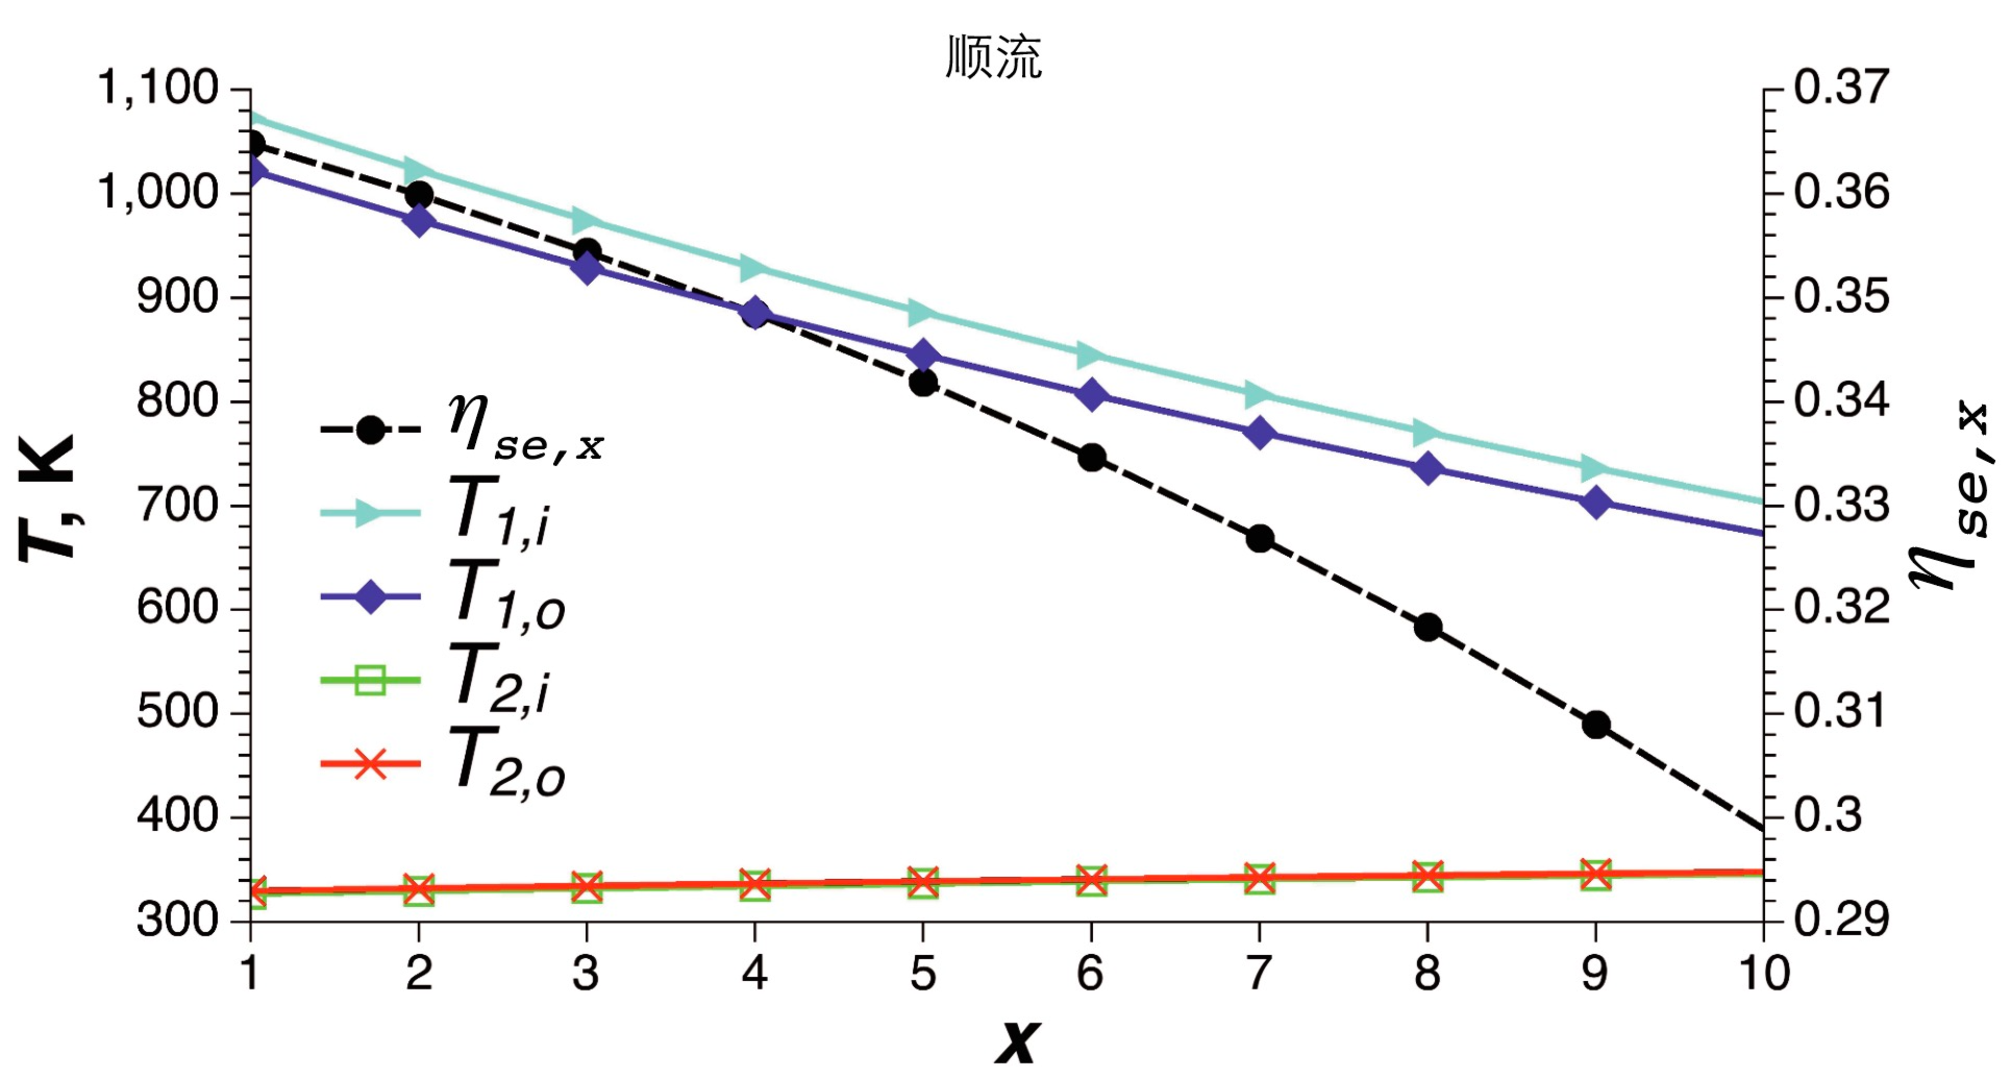
\includegraphics[width = 0.45\columnwidth, angle = 0]{fig/Parallelflow}}
%	\subfigure[Counterflow]{
%	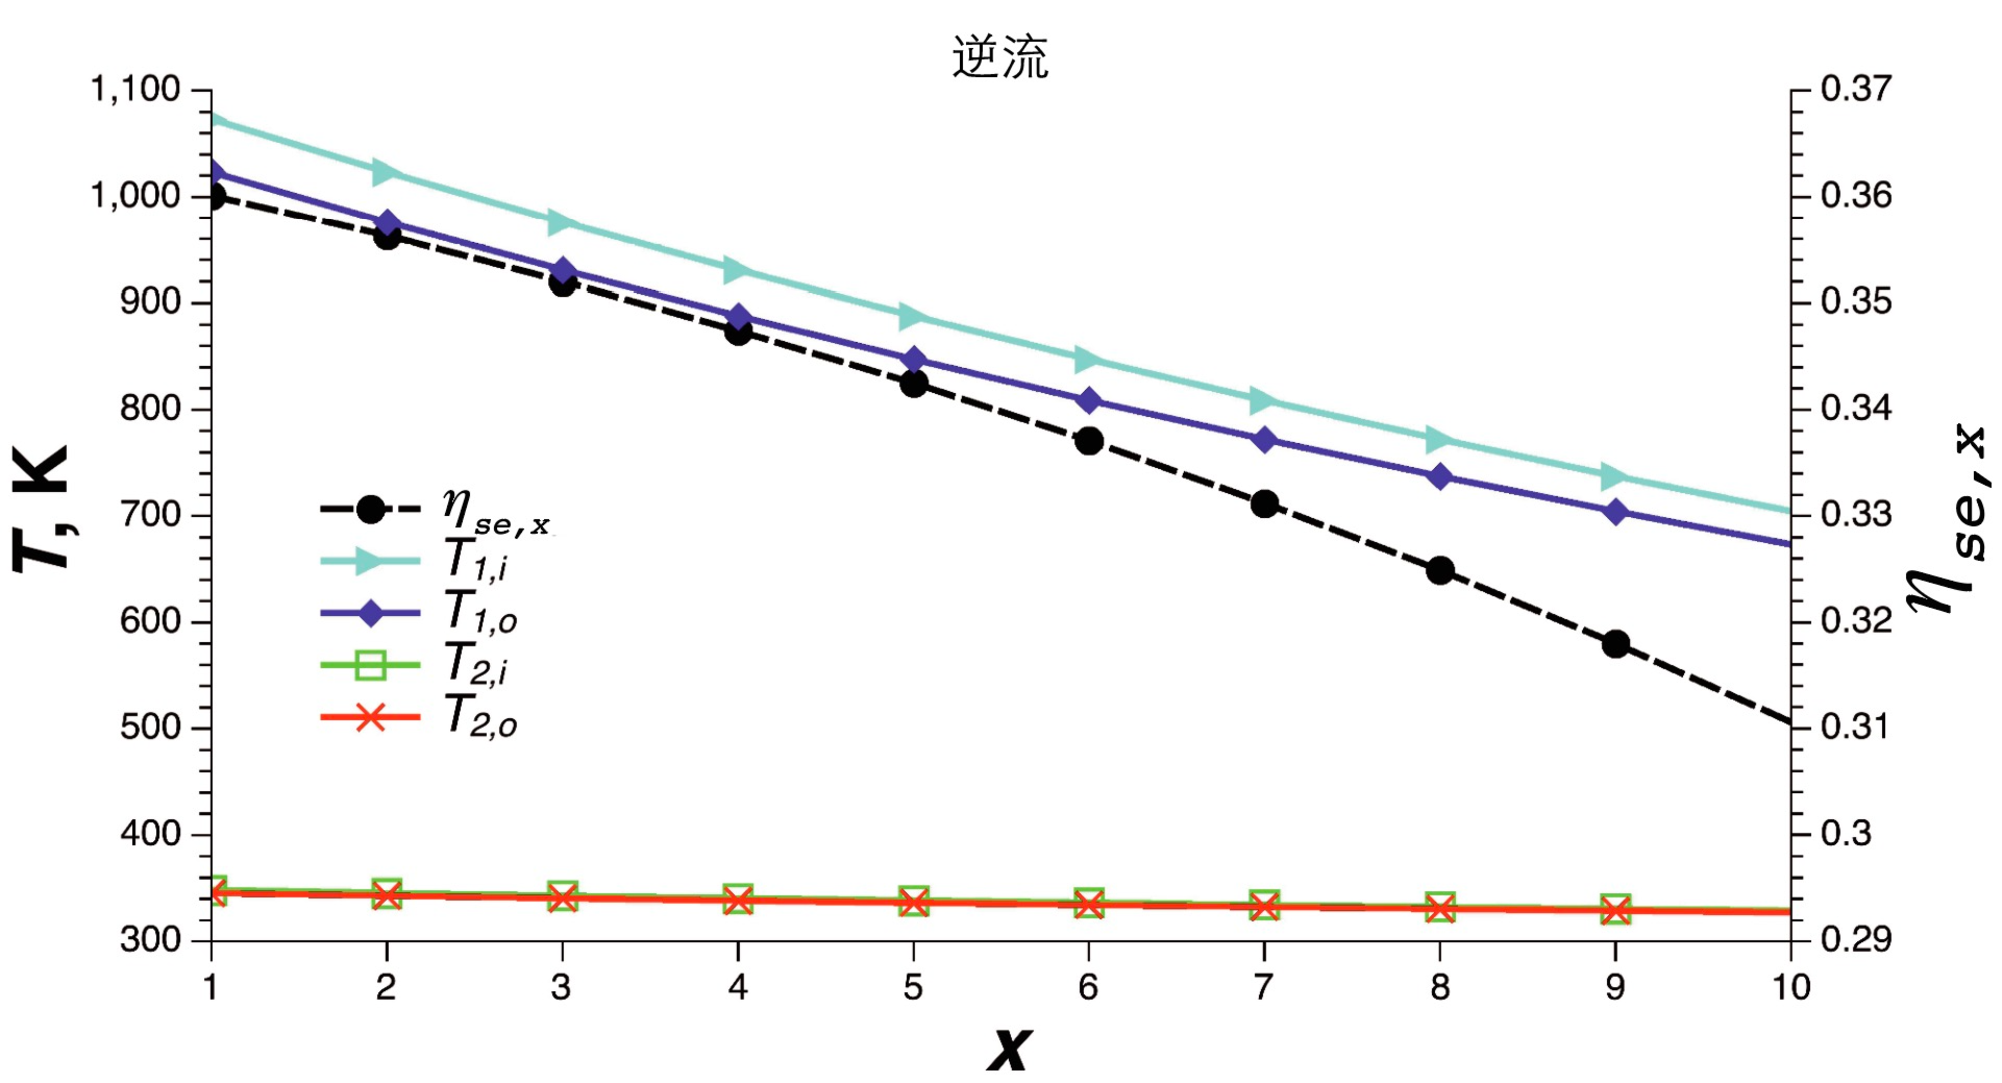
\includegraphics[width = 0.45\columnwidth, angle = 0]{fig/Counterflow}}
%	\caption{Temperature series of two fluids and efficiency of Stirling engines in column $x$}
%	\label{fig:ParallelflowAndCounterflow}
%\end{center}
%\end{figure}

\noindent \begin{figure}[htbp]
\begin{center}
	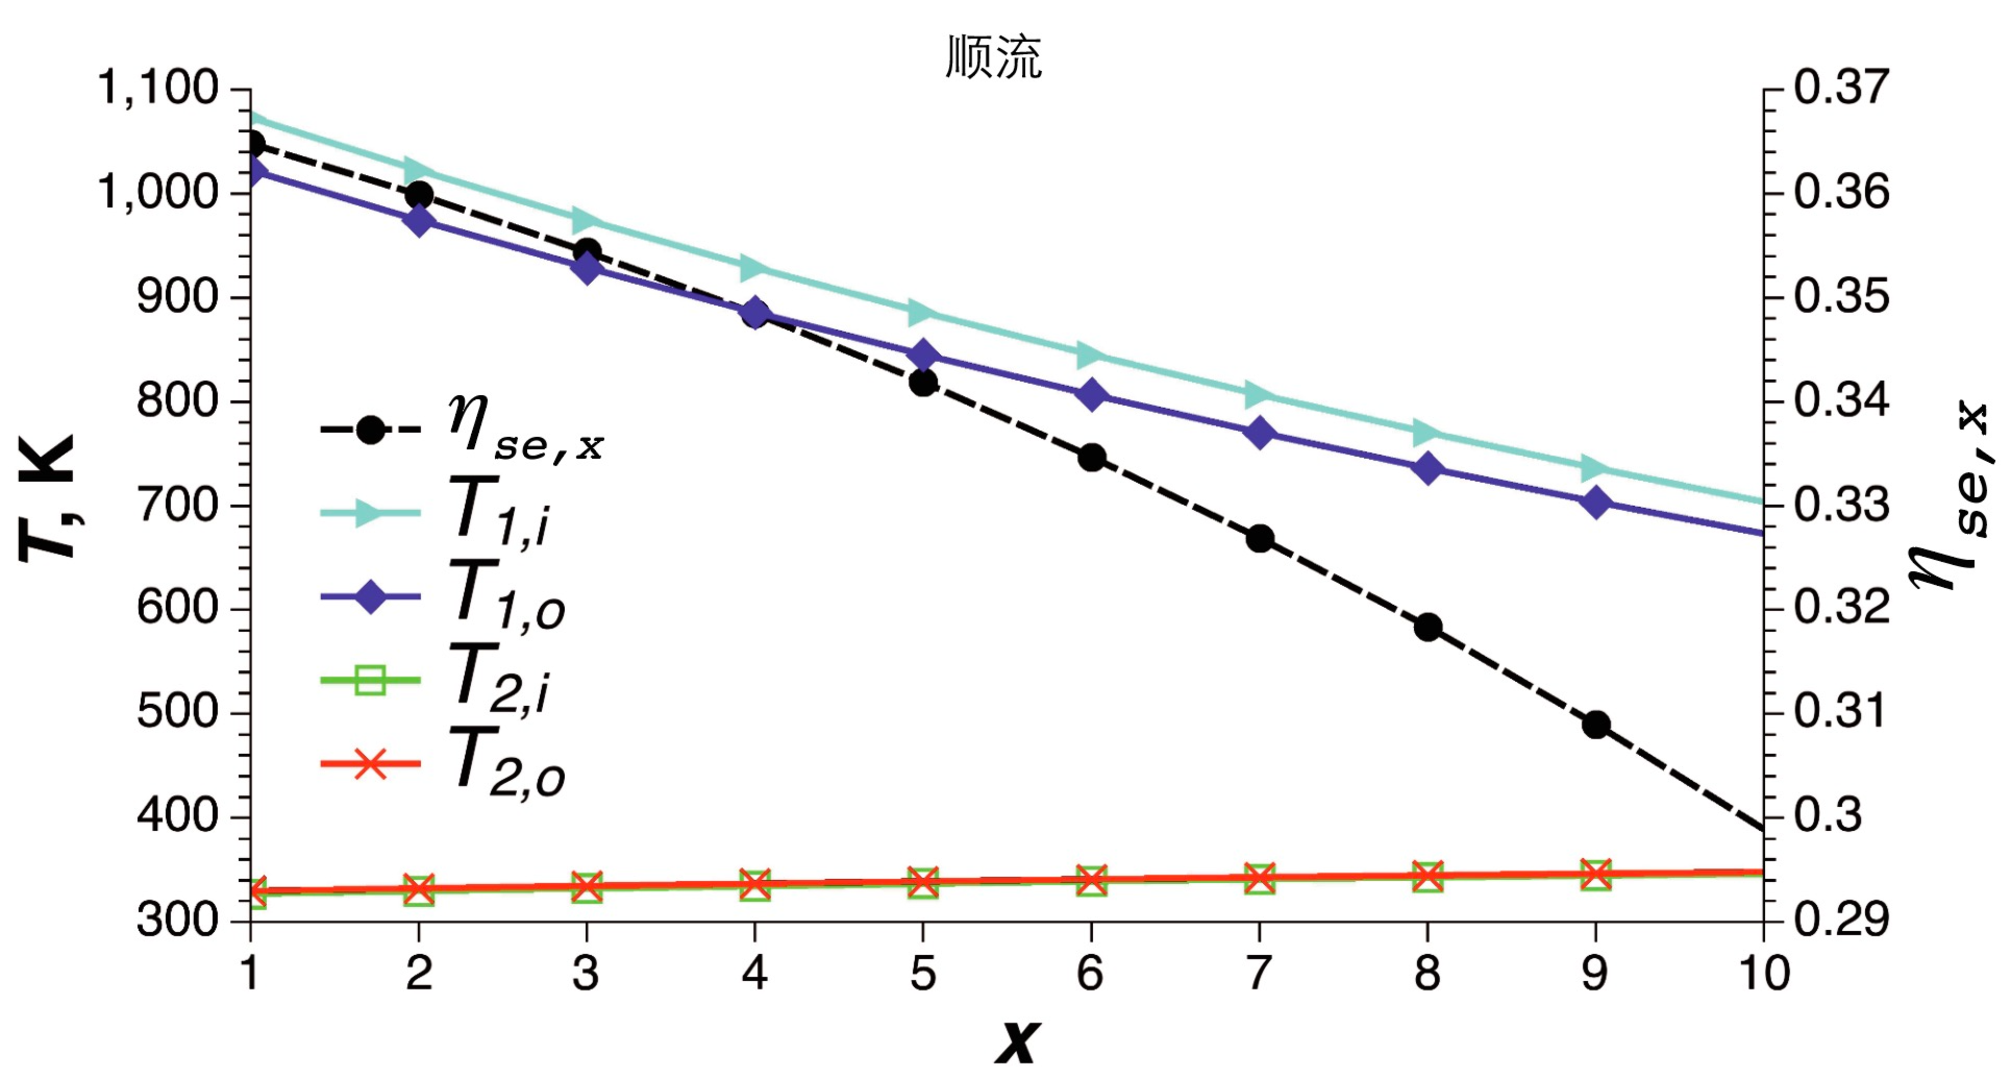
\includegraphics[width = 0.8\columnwidth, angle = 0]{fig/Parallelflow}
	\caption{Parallel flow: Temperature series of two fluids and efficiency of Stirling engines in column $x$}
	\label{fig:Parallelflow}
\end{center}
\end{figure}
\noindent \begin{figure}[H]
\begin{center}
	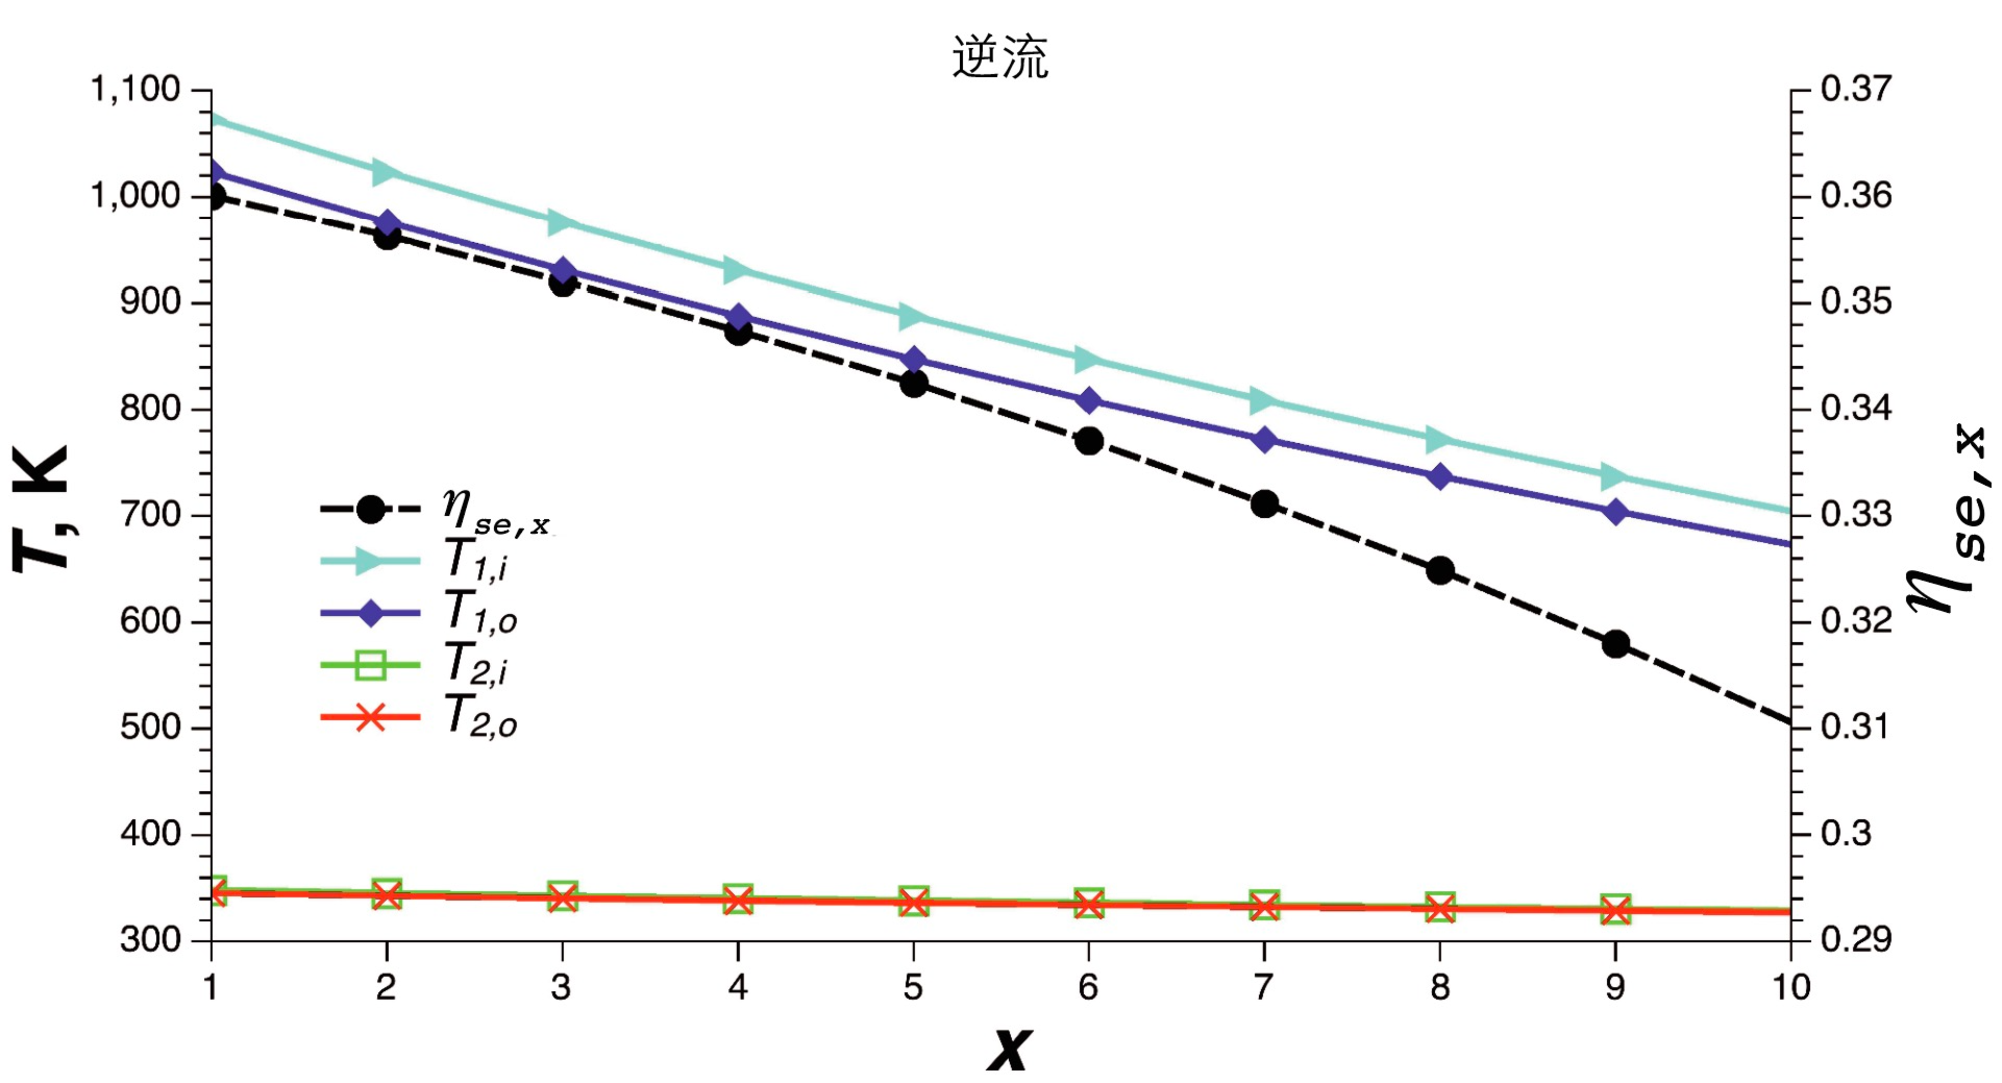
\includegraphics[width = 0.8\columnwidth, angle = 0]{fig/Counterflow}
	\caption{Counterflow: Temperature series of two fluids and efficiency of Stirling engines in column $x$}
	\label{fig:Counterflow}
\end{center}
\end{figure}

It can be concluded that the temperature increment of cooling fluid is much smaller than the temperature decrement of heating fluid due to their large difference of $c_p\dot{m}$, which leads to a small difference of overall efficiency of Stirling engine array between the two flow types.

To find out a clear difference of the two flow types, a simple model of Stirling engine array was developed with air as the heating fluid and water as the cooling fluid. $T_{1,i}, T_{1,o}, T_{2,i}, q_{1,m}$ are fixed and chosen the same values as in the cascade system. Change the value of $q_{2,m}$, and the corresponding Stirling engine array efficiency of the two flow types ($\eta_p$ and $\eta_c$) can be obtained. Figure~\ref{fig:SEAflowtypes} shows the efficiency of Stirling engine array with different $q_{2,m}$ in two flow types. It can be found that counterflow has a higher efficiency than parallel flow, and with lower $q_{2,m}$ comes with higher efficiency difference.
\nomenclature[S]{$p$}{Parallel flow}
\nomenclature[S]{$c$}{Counterflow}

For a system with large difference of $c_p\dot{m}$ of two fluids, that means one fluid can only achieve a small temperature rise (drop) compared to the other fluid, will lead to a small difference of two flow types. For a system with similar difference of $c_p\dot{m}$, use the counterflow can achieve a higher efficiency.

\noindent \begin{figure}[H]
\begin{center}
	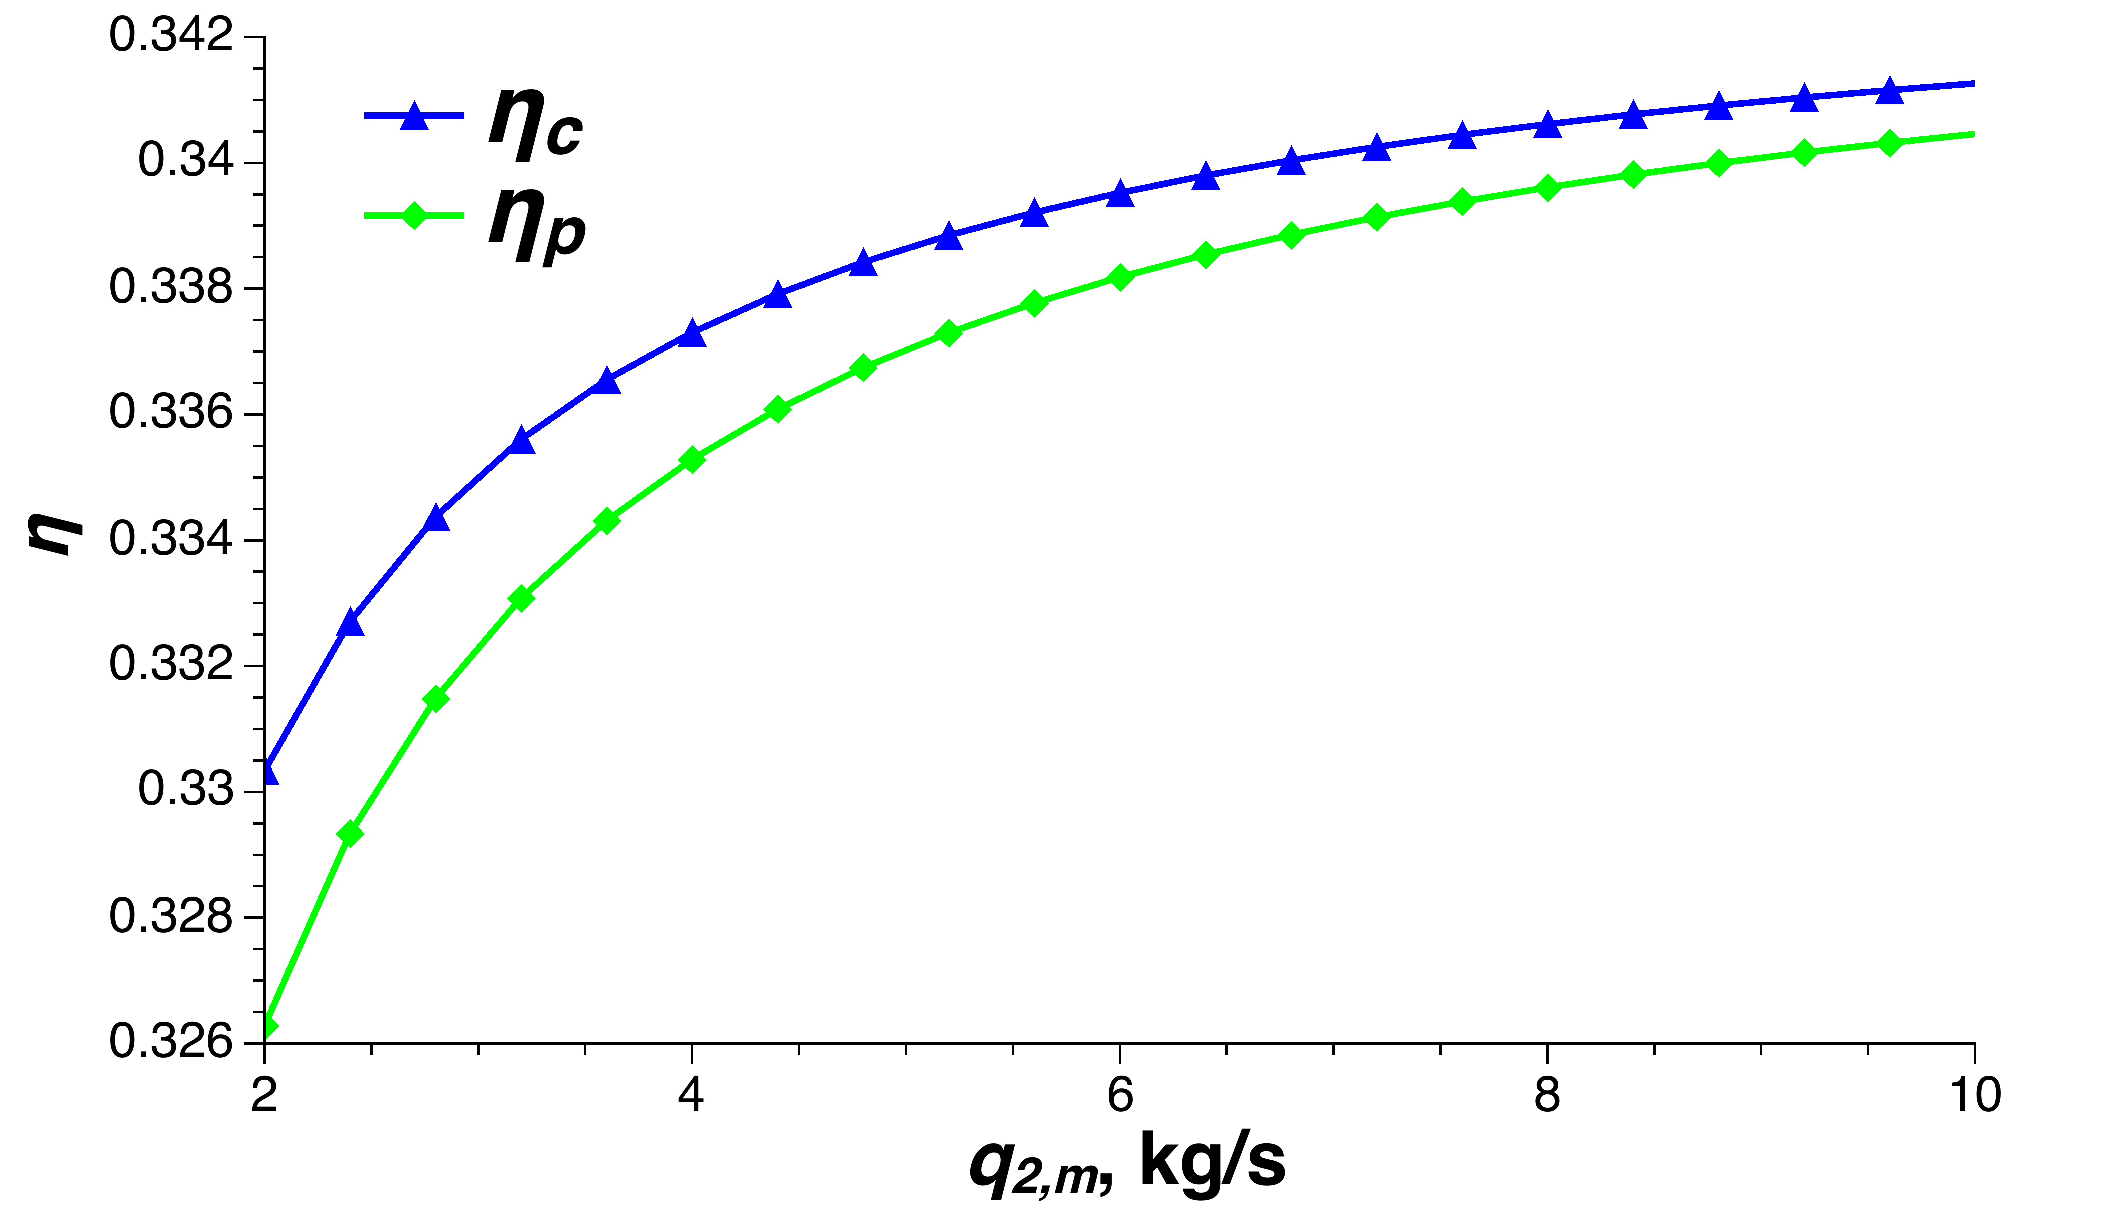
\includegraphics[width = 0.8\columnwidth, angle = 0]{fig/SEAflowtypes}
	\caption{Efficiency of Stirling engine array with different $q_{2,m}$}
	\label{fig:SEAflowtypes}
\end{center}
\end{figure}
%\section{System evaluation}

\section{Conclusion}

In this chapter, an effective typical cascade system proposed in Chapter~\ref{cha:SystemTopology} is chosen for evaluation. 
This cascade system uses two different types of collectors and two different power generation methods. 
Steam Rankine cycle is applied for this system for its widely applied applications.
Reasonable parameters are selected and the system model was developed.
Two stand-alone systems are chosen as the comparison systems for system evaluation. 
They use the same dish collectors and trough collectors of the cascade system. 
Simulations of the cascade system were carried out and results were compared with corresponding stand-alone systems.

Results show that $I_r$ is the key factor to determine whether cascade system should be applied in a certain location. Compared to corresponding stand-alone systems, the cascade system can achieve a higher efficiency with high solar irradiance ($I_r > 550\,\mathrm{W/m^2}$). The directions to increase the efficiency difference between cascade system and corresponding stand-alone systems were also considered. To design a cascade system including Stirling engine array, flow type of fluids for heating and cooling Stirling engine array is also required to be considered. 

%However, it has to be pointed out that this thesis uses a simple Stirling cycle efficiency formula given in the book~\cite{Stine1985}. This formula takes no consideration of various losses and irreversibilities, such as pressure drop, shuttle conduction, finite speed of piston and mechanical friction. The heat transfer process between the fluids and the Stirling engines has been simplified to be constant heat transfer coefficient. However, the imperfect model of the Stirling engine doesn't affect the idea of solar thermal cascade system presented in this thesis. More accurate Stirling engine model can be applied to achieve higher accuracy of the system in the future work. Besides, a cascade system with a different $\beta$ not only affects the efficiency of the system but also changes the portion of dish collector area to the total collector area, which will affect the cost. The cost analysis and optimization research of the cascade system is not included in this thesis, which are worthy candidates for further research.